The prevailing description of nature at the fundamental level is a relativistic quantum field theory called the Standard Model (SM). Developed in the latter half of the 20th century, the SM has seen extraordinary success in its predictive power and is widely considered the most rigorously tested physical theory. The characteristics of the SM proceed from symmetries embedded in the Lagrangian of the theory. At the heart of the SM are the local gauge transformations associated with the gauge group product: 
\begin{equation}
    \SUthreeC \times \SUtwoW \times \UoneY,
\end{equation}
where the subscript on each gauge group identifies an associated conserved quantity: color charge C, weak isospin W, and weak hypercharge Y (all detailed in Section~\ref{sec:Forces}), which generate three of the four fundamental forces of nature (electromagnetic, weak, and strong; gravity is absent in the SM). Adding a collection of 17 quantized fields (by one way of counting) that respect this symmetry completes the SM. Experiments have revealed that the constituant building blocks of the universe are point-like particles, understood in the SM as excitations in the quantum fields, with each observed ``matter'' particle corresponding to an excitation in one of 12 fields, listed in detail in Section~\ref{sec:Particles}. Interactions among particles by the three fundamental forces are understood as the exchange of ``virtual'' particles, excitations in one of four fields, reviewed in Section~\ref{sec:Forces}. The remaining field corresponds to the Higgs particle and is responsible for the masses of the other particles, explained in Section~\ref{sec:Higgs}. 

\subsection{Elementary particles} \label{sec:Particles}
Localized excitations, or quanta, of the quantum fields in the SM are called elementary particles. Particles are observed either directly or indirectly through experiment and carry intrinsic properties that distinguish them from one another, such as electric charge, mass, and quantum numbers like spin. Every particle has a corresponding antiparticle, which, roughly speaking, is identical to the particle save for its carrying some opposite quantum numbers, e.g., electric charge for charged particles. All SM particles (and antiparticles) can be classified as either fermions or bosons, depending on their spin quantum number, detailed below in Sections~\ref{sec:Fermions} and~\ref{sec:Bosons}. Provided in Fig.~\ref{fig:SM} is a diagram of all the particles in the SM, practically organized, and includes a number of important properties for each; this diagram may be used as a map of the theory described in the following Sections.

\begin{figure}[H]
    \centering
    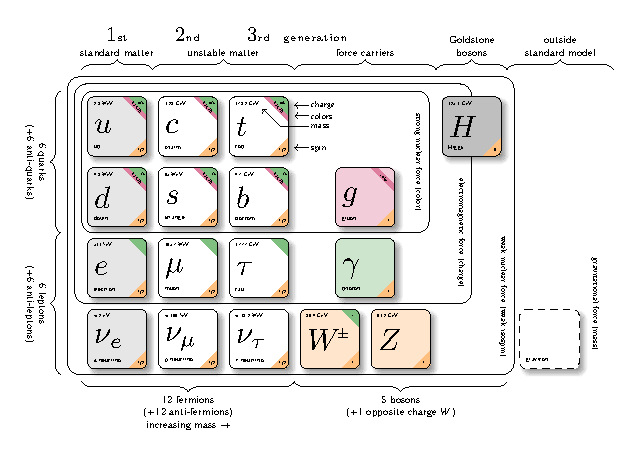
\includegraphics[width=1\textwidth]{Images/model-physics.pdf}
    \caption{Every elementary particle in the SM}
    \label{fig:SM}
\end{figure}

\subsubsection{Fermions} \label{sec:Fermions}
%fermions

Particles with half-integer spin quantum numbers obey Fermi-Dirac spin-statistics, which prevents any two identical particles from occupying the same state in a system at thermodynamic equilibrium, leading to the famous Pauli exclusion principle. Particles following a Fermi-Dirac distribution are given the eponymous name fermions, and while they are a general classification of any particle with half-integer spin, within the SM, fermions refer to a specific set of massive, interacting, ``matter'' particles that are subdivided into two key types: leptons and quarks. 

%leptons

Leptons $\ell$ are spin 1/2 fermions that can be electrically charged or neutral and interact via the weak nuclear force; they do not interact via the strong nuclear force (see Sections~\ref{sec:WeakInteraction} and~\ref{sec:StrongInteraction}). There are six types, or flavors, of leptons: the electron $e^-$, muon $\mu^-$, tau $\tau^-$, electron neutrino $\nu_e$, muon neutrino $\nu_{\mu}$, and tau neutrino $\nu_{\tau}$. These can be grouped into three generations: electronic, muonic, and tauonic, each with an electrically charged lepton and an electrically neutral lepton, dubbed a neutrino. Each lepton carrys a lepton family quantum number $L_e$, $L_{\mu}$, or $L_{\tau}$, equal to 1 ($-1$ for antileptons), that is approximately conserved (neutrino oscillations violate this). What is always conserved in interactions is lepton number $L = n_{\ell}-n_{\overline{\ell}}$, where $n_{\ell}$ and $n_{\overline{\ell}}$ are the number of leptons and antileptons at the start or end of an SM process.

An important characteristic of both fermions and bosons is their helicity, being the sign of the projection of a particle's spin onto its momentum: ``right-handed'' if the spin and momentum vectors align ($+1$), ``left-handed'' if the vectors are opposed ($-1$), denoted with an $R$ or $L$ subscript, respectively. In the limit where the particle is massless, helicity is essentially chirality, an intrinsic property of a particle that determines the representation it transforms under (for this reason we refer to left-handed and right-handed particles as chiral). Each generation of left-handed leptons form a weak isospin doublet with $T=1/2$:
\begin{equation}
    \left(\begin{array}{c}
        \nu_e \\
        e^-
    \end{array}\right)_L,
    \left(\begin{array}{c}
        \nu_{\mu} \\
        \mu^-
    \end{array}\right)_L,
    \left(\begin{array}{c}
        \nu_{\tau} \\
        \tau^-
    \end{array}\right)_L
\end{equation} 
while the right-handed leptons form singlets: $e^-_R$, $\mu^-_R$, $\tau^-_R$ with $T=0$. Note that there are no right-handed neutrinos in the SM, and that only left-handed leptons participate in charged weak interactions. For antileptons, the inverse is true: there are only right-handed antineutrinos and only right-handed charged antileptons participate in weak interactions.

Leptons are initially massless in the SM. Charged leptons aquire mass via the Higgs mechanism, while neutrinos remain massless. No neutrino mass has ever been measured (although upper bounds have been placed); however, observations of neutrino flavor oscillations confirm that neutrinos do indeed have very small masses, contrary to the SM. Table~\ref{tab:Leptons} lists for each lepton the flavor, spin, lepton family number, electric charge $Q$, weak isospin $T_3$, weak hypercharge $Y_W$, and observed mass (or upper bound on the mass for the neutrinos). There is a corresponding antiparticle for each lepton, where the charges are sign-flipped but retain the same mass.
\begin{table}[H]
    \begin{center}
        \caption{Quantum numbers and masses of the SM leptons. This table only lists the properties of left-handed leptons, with right-handed antileptons forming a similar table with the charges sign-flipped.}
        \begin{tabular}{lrrrrrrrl}
            \hline \hline
            Flavor          & Spin  & $L_e$ & $L_{\mu}$ & $L_{\tau}$    & $Q$   & $T_3$     & $Y_W$ & Obs. mass [MeV] \\ \hline
            $e$             & $1/2$ & $+1$   & $0$       & $0$           & $-1$   & $-1/2$    & $+1$  & \;\;\;\;$\num{0.511}$ \\
            $\mu$           & $1/2$ & $0$   & $+1$       & $0$           & $-1$   & $-1/2$    & $+1$  & \;\;\;\;$\num{105.7}$ \\
            $\tau$          & $1/2$ & $0$   & $0$       & $+1$           & $-1$   & $-1/2$    & $+1$  & \;\;\;\;$\num{1.777e3}$ \\
            $\nu_e$         & $1/2$ & $+1$   & $0$       & $0$           & $0$   & $+1/2$    & $-1$  & $<\num{2.2e-6}$ \\
            $\nu_{\mu}$     & $1/2$ & $0$   & $+1$       & $0$           & $0$   & $+1/2$    & $-1$  & $<\num{0.17}$ \\
            $\nu_{\tau}$    & $1/2$ & $0$   & $0$       & $+1$           & $0$   & $+1/2$    & $-1$  & $<\num{15.5}$ \\ \hline \hline
        \end{tabular}
        \label{tab:Leptons}
    \end{center}
\end{table}



%quarks

Quarks $q$ are chiral spin 1/2 fermions that carry fractional electric charge (in multiples of 1/3), weak isospin and weak hypercharge, and—--unique among the SM fermions---interact with the strong force. Analogous to lepton number, quarks carry a baryon quantum number $B$ of 1/3. Baryon number is strictly conserved in the SM, and---for any interaction---is defined as $3B=n_q-n_{\overline{q}}$, where $n_q$ and $n_{\overline{q}}$ are the number of quarks and antiquarks at the start or end of a process. Remarkably, quarks---identical to leptons---come in six flavors that can likewise be grouped into three generations (this unexplained parallel partly motivates the search for new physics in this thesis). The quark flavors are: up $u$ and down $d$ (first-generation), charm $c$ and strange $s$ (second-generation), and top $t$ and bottom $b$ (third-generation). Also, similar to leptons, quarks aquire mass via the Higgs mechanism. Table~\ref{tab:quarks} lists the quantum numbers and masses of each flavor of quark.
\begin{table}[H]
    \begin{center}
        \caption{Quantum numbers of quarks. Color charges are not considered. This table only lists the properties of quarks, with antiquarks forming a similar table with the charges sign-flipped.}
        \begin{tabular}{lrrrrrl}
            \hline \hline
            Flavor   & Spin  & $B$   & $Q$       & $T_3$     & $Y_W$   & Obs. Mass [MeV] \\ \hline
            up       & $1/2$ & $1/3$ & $+2/3$    & $-1/2$    & $+1/3$  & $\num{2.3}$ \\
            down     & $1/2$ & $1/3$ & $-1/3$    & $-1/2$    & $+1/3$  & $\num{4.8}$ \\
            charm    & $1/2$ & $1/3$ & $+2/3$    & $-1/2$    & $+1/3$  & $\num{1.274e3}$ \\
            strange  & $1/2$ & $1/3$ & $-1/3$    & $+1/2$    & $+1/3$  & $\num{9.5e1}$ \\
            top      & $1/2$ & $1/3$ & $+2/3$    & $+1/2$    & $+1/3$  & $\num{1.73210e5}$ \\
            bottom   & $1/2$ & $1/3$ & $-1/3$    & $+1/2$    & $+1/3$  & $\num{4.180e3}$ \\ \hline \hline
        \end{tabular}
        \label{tab:quarks}
    \end{center}
\end{table}

Each flavor of quark transforms as a color triplet under \SUthreeC, meaning it has a red, blue, or green color charge (antired, antiblue, or antigreen for antiquarks). As a quark absorbs or emits a gluon (carrying a color-anticolor charge), its color charge will change correspondingly. Quarks combine via the strong interaction to form color-neutral hadrons that are either a quark-antiquark pair called a meson (e.g., a pion) or a combination of three quarks called a baryon (e.g., the proton and the neutron). Color confinement restricts quarks inside of hadrons, and in the instance of a free quark (or gluon), QCD matter will spontaneously be pulled from the vacuum to neutralize the bare color charge, a process known as hadronization. Hard proton-proton collisions as seen in the LHC will often emit quarks, which must undergo hadronization repeatedly until all color fragments are neutralized, generating a slew of mesons and baryons all traveling within a tight cone with the momentum of the original quark. These cones of hadrons, colloquially called jets, are ubiquitous in collider experiments and are essential ingredients in many physics analyses. 


\subsubsection{Bosons} \label{sec:Bosons}
The spin statistics of particles with integer-valued spin quantum numbers follow a Bose-Einstein distribution, which allows an arbitrary number of identical particles to occupy quantum states and maintain thermal equilibrium (as opposed to Fermi-Dirac statistics). Particles with this behavior are naturally called a bosons. After the SM fermions, a collection of four SM bosons constitute the remainder of all observed fundamental particles. SM bosons can be massive or massless and are responsible for mediating the interactions between all particles. As the local gauge transformations of the SM are responsible for the fundamental interactions, the associated bosons are often called gauge bosons. In the SM there are three types of vector (spin 1) gauge bosons: the photon, the weak bosons, and the gluons; and one scalar (spin 0) boson: the Higgs boson. 

The photon is a massless spin 1 gauge boson that mediates the electromagnetic force, meaning it couples to any fermion with an electric charge (all but neutrinos). Photons themselves are uncharged, so they do not self-interact. The weak gauge bosons are also spin 1 and mediate the weak force. There are three kinds of weak gauge bosons: two charged, $W^+$ and $W^-$, and one neutral, $Z^0$. They are all massive, aquiring their masses via the Higgs mechanisim as explained in Section~\ref{sec:Higgs}. There are eight Gluons, massless spin 1 gauge bosons that mediate the strong force between particles with color charge, i.e., quarks. Gluons carry color charge and thus self-interact, leading to color confinemnt. The Higgs boson is a massive, complex scalar boson that is responsible for providing mass to the gauge bosons and SM fermions, through different mechanisms. The Higgs is theorized to self-interact and in 2012 was the last SM particle to be discovered. 


\subsection{Fundamental interactions} \label{sec:Forces}

\subsubsection{The electromagnetic interaction} \label{sec:EMInteraction}

%Electrically charged particles, such as electrons, quarks, and the $W^{\pm}$ bosons, to name a few, interact via 
The Electromagnetic (EM) interaction is described in the SM by an Abelian gauge theory called Quantum Electrodynamics (QED) with the gauge group \Uone. The \Uone symmetry allows a gauge transformation of the EM vector field $A^{\mu}$ to be made:
\begin{equation}
    A^{\mu} \rightarrow A'^{\mu} = A^{\mu} + \partial^{\mu}\chi
\end{equation}
with no change to the free-field lagrangian. Allowing the EM field to couple to (interact with) electrically charged Dirac fermions $\psi$, while imposing invariance on the whole QED lagrangian (free field + interacting terms), requires a simultaneous (and local) phase transformation of $\psi$:
\begin{equation}
    \psi \rightarrow \psi' = e^{-ie\chi(x)}\psi
\end{equation}
with the factor $e$ on the phase being the experimentally measured charge of the electron (related to the coupling strength of $A^{\mu}$ to $\psi$). These gauge transformations forbid any mass and self-interacting terms of $A^{\mu}$ from appearing in the QED lagrangian, and restrict the quanta of $A^{\mu}$ to vector bosons. Photons are consistent with the constraints of the \Uone~symmetry of QED (being massless spin 1 bosons that do not self-interact) and were confirmation that QED was an accurate description of the EM force. As with the other two forces in the SM, we say that the photon ``mediates'' EM interactions between particles charged under QED, as the photon's coupling to electrically charged particles is responsible for the forces between them. For example, the Feynman diagram in Fig.~\ref{fig:QEDFeynmanDiagram} shows the electromagnetic repulsion of two electrons propogating through space-time by the exchange of a virtual photon, the mediator of the EM force. 
\begin{figure}[H]
    \centering
    \vspace{0.05\textwidth}
    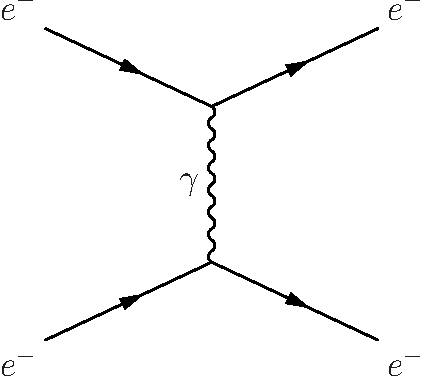
\includegraphics[width=0.3\textwidth]{Images/Theory/QEDInteraction.pdf}\hspace{0.1\textwidth}
    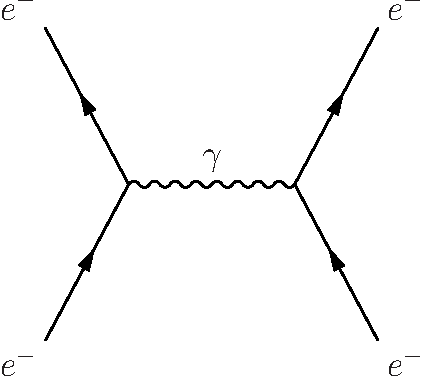
\includegraphics[width=0.3\textwidth]{Images/Theory/QED_s_channel.pdf}\vspace{0.05\textwidth}
    \caption{Left: A tree-level Feynman diagram in the t-channel showing two electrons interacting (repelling) via the exchange of a virtual photon. Right: Rotating the t-channel diagram 90 degrees gives the s-channel diagram, showing the annihilation of an electron-antielectron pair into a virtual photon, which propagtes before decaying again into an electron-antielectron pair. Both phenomena are described with QED.}
    \label{fig:QEDFeynmanDiagram}
\end{figure}
At very high energies (such as shortly after the big bang) the EM interaction is understood to be unified with the weak interaction, collectively called the electroweak force, that is only broken into separate forces at a temperature of approximately \SI{e15}{K} (explained in more detail in Section~\ref{sec:WeakInteraction}).

\subsubsection{The weak interaction} \label{sec:WeakInteraction}

%The weak force is responsible for the transition of particles from one flavor to another, e.g., radioactive beta decay, muon decay. While Quantum Flavordynamics (QFD) can describe the weak interaction, it is better modeled with Electroweak Theory (EWT). EWT is a unified theory of electromagnetic and weak interactions and is represented as a Yang-Mills field with an SU(2) $\times$ U(1) gauge group. 

%The gauge fields of EWT interact with weak isospin $T$ and weak hypercharge $Y$,


%Three isospin fields $W_1$, $W_2$, and $W_3$, and the weak hypercharge field $B$

Weak interactions are best described in a unified framework with electromagnetism called Electroweak Theory (EWT). The gauge fields of EWT are the weak isospin triplet $W^i_{\mu}$ ($i = 1, 2, 3$) and the weak hypercharge field $B_{\mu}$ which are symmetric under the gauge group $\SUtwo \times \UoneY$. (The Y subscript of \UoneY distinguishes this symmetry from the $\Uone_{\text{EM}}$ symmetry of QED.) These four fields correspond to the unphysical gauge bosons of EWT: the \PWewt{1}, \PWewt{2}, \PWewt{3}, and \PBewt bosons, all of which are massless. 

Spontaneous symmetry breaking of EWT results in the manifestation of the physical bosons of the weak and electromagnetic interactions.
Electric charge $Q$ is the unique linear combination of weak isospin $T$ and weak hypercharge \YW:
\begin{equation}
    Q = \Tthree +\frac{1}{2}\YW
\end{equation}
The neutral weak boson \PZzero and the photon \Pgamma are a linear combination of the \PWewt{3} and \PBewt bosons:
\begin{equation}
    \left(
    \begin{matrix}
        \Pgamma \\
        \PZzero
    \end{matrix}
    \right)
    =
    \left(
    \begin{matrix}
        \cos\weakangle & \sin\weakangle \\
        -\sin\weakangle & \cos\weakangle
    \end{matrix}
    \right)
    \left(
    \begin{matrix}
        \PBewt \\
        \PWewt{3}
    \end{matrix}
    \right)
\end{equation} 
where the parameter \weakangle is the weak mixing angle. The \PWewt{1} anmd \PWewt{2} bosons likewise combine to form the charged weak bosons \PWpm according to the complex linear combination:
\begin{equation}
    \left(
    \begin{matrix}
        \PWplus \\
        \PWminus
    \end{matrix}
    \right)
    =
    \frac{1}{\sqrt{2}}
    \left(
    \begin{matrix}
        1 & -i \\
        1 & i
    \end{matrix}
    \right)
    \left(
    \begin{matrix}
        \PWewt{1} \\
        \PWewt{2}
    \end{matrix}
    \right).
\end{equation}
The weak bosons aquire mass from the Higgs field, while the photon remains massless. 



\subsubsection{The strong interaction} \label{sec:StrongInteraction}
The strong force emerges from the \SUthreeC~gauge group of the SM which is described by the non-abelian gauge theory called Quantum Chromodynamics (QCD). The \SUthreeC~symmetry of QCD generates eight massless vector (spin 1) gauge bosons called gluons, the carriers of the strong force, that exclusively interact with particles carrying ``color'' charge: either red, blue, green, antired, antiblue, or antigreen. Of the fermions, only quarks carry color charge and interact with gluons. As gluons themselves carry a color and anticolor charge, they self-couple and may interact at four- and three-point vertices. This self-interaction among the force-carrying gluons prevents any energy fall-off between two color-charged quarks as the distance between them increases. At a certain distance of separation, the binding energy becomes so large that it is energetically favorable to produce two new quarks from the vaccum to bind to the original, separated quarks, and form two color-neutral hadrons rather than two ``free'' or color-bare quarks. This phenomenon is called confinement, and is responsible for the hadronization of free quarks into jets, and why it is impossible to observe a free quark; quarks will always be observed in bound states as hadrons (see Section~\ref{sec:Fermions}).
The beta function of QCD, which charts how the strong coupling constant $\alpha$ varies with energy scale (or inversely, interaction distance) is given by:
\begin{equation}
    \beta_1(\alpha) = \frac{\alpha_s^2}{\pi}\left(-\frac{11N}{6}+\frac{n_f}{6}\right)
\end{equation}
with $N=3$ for the \SUthree~gauge of QCD, and $n_f$ the number of quark-like fermions. As long as $n_f<16$, which experiment has so far confirmed (only six known quarks in the SM have been observed), the beta function is negative and is asymptotically free, i.e., the coupling strength of QCD decreases with the energy scale of the interaction. Asymptotic freedom allows for the binding of protons together with neutrons within the close-proximity of an atomic nucleus, on the order of 1-3 fm, and likewise the binding of quarks within protons and neutons (and other hadrons), on the order of $<$ 0.8 fm. 

\subsubsection{The Higgs field} \label{sec:Higgs}
The Higgs field $\phi$ is a complex scalar field with a potential $V(\phi)$ of the form:
\begin{equation}
    V(\phi) = -\frac{1}{2}\mu^2|\phi|^2 + \frac{1}{4}\lambda|\phi|^4,
\end{equation}
where $\lambda$ and $\mu$ are parameters (ultimately related to the Higgs self-coupling and Higgs mass). The potential has the famous ``mexican hat'' shape, symmetric about rotations in $\phi$, with a non-zero minimum expectation value $\braket{\phi} \neq 0$, as seen in the graph in Fig.~\ref{fig:HiggsPotential}. Initially, the Higgs potential exisits in the unstable state where $\braket{\phi} = 0$, preserving the $\phi$ symmetry. A fluctuation in the Higgs field will minimize the potential as $\phi$ aquires some non-zero vacuum expectation value (VEV) $\braket{0|\phi|0} = v$, and in doing so breaks the rotational symmetry of $\phi$; this is called spontaneous symmetry breaking. It is convenient to now parameterize $\phi$ in terms of two real scalar fields $h$ and $\chi$ and expand about $v$, like:
\begin{equation}
    \phi = \frac{1}{\sqrt{2}}(v+h)e^{i\chi/v},
\end{equation}
and after substituting the fields back into the lagrangian, we emerge with a massive physical higgs boson $h$ and a massles ``Goldstone'' boson $\chi$.

In EWT, the spontaneous symmetry breaking of the Higgs field is embedded in the $\SUtwoW\times\UoneY$ local gauge symmetry, where the Higgs field is now a weak isospin doublet. In a similar way to the above example, the electroweak symmetry is broken, and we are left with a massive Higgs field, and four massles Goldstone bosons. Through chosing a gauge, the Goldstone bosons are ``eaten'' and we are left with the physical gauge bososns of EWT: a massles photon and three massive weak gauge bosons. 

The SM fermions couple to the Higgs field with so-called Yukawa couplings, like $\overline{\ell}_L\phi e_R$, $\overline{q}_L\phi d_R$, and $\overline{q}_L\tilde{\phi}u_R$ which form weak isospin singlets. After spontaneous symmetry breaking of the Higgs field, the fermions aquire masses in a similar way to the gauge bosons, while the absence of any right-handed neutrinos in the SM prevents them from coupling to the Higgs field and leaves them massless.

\begin{figure}[H]
    \centering
    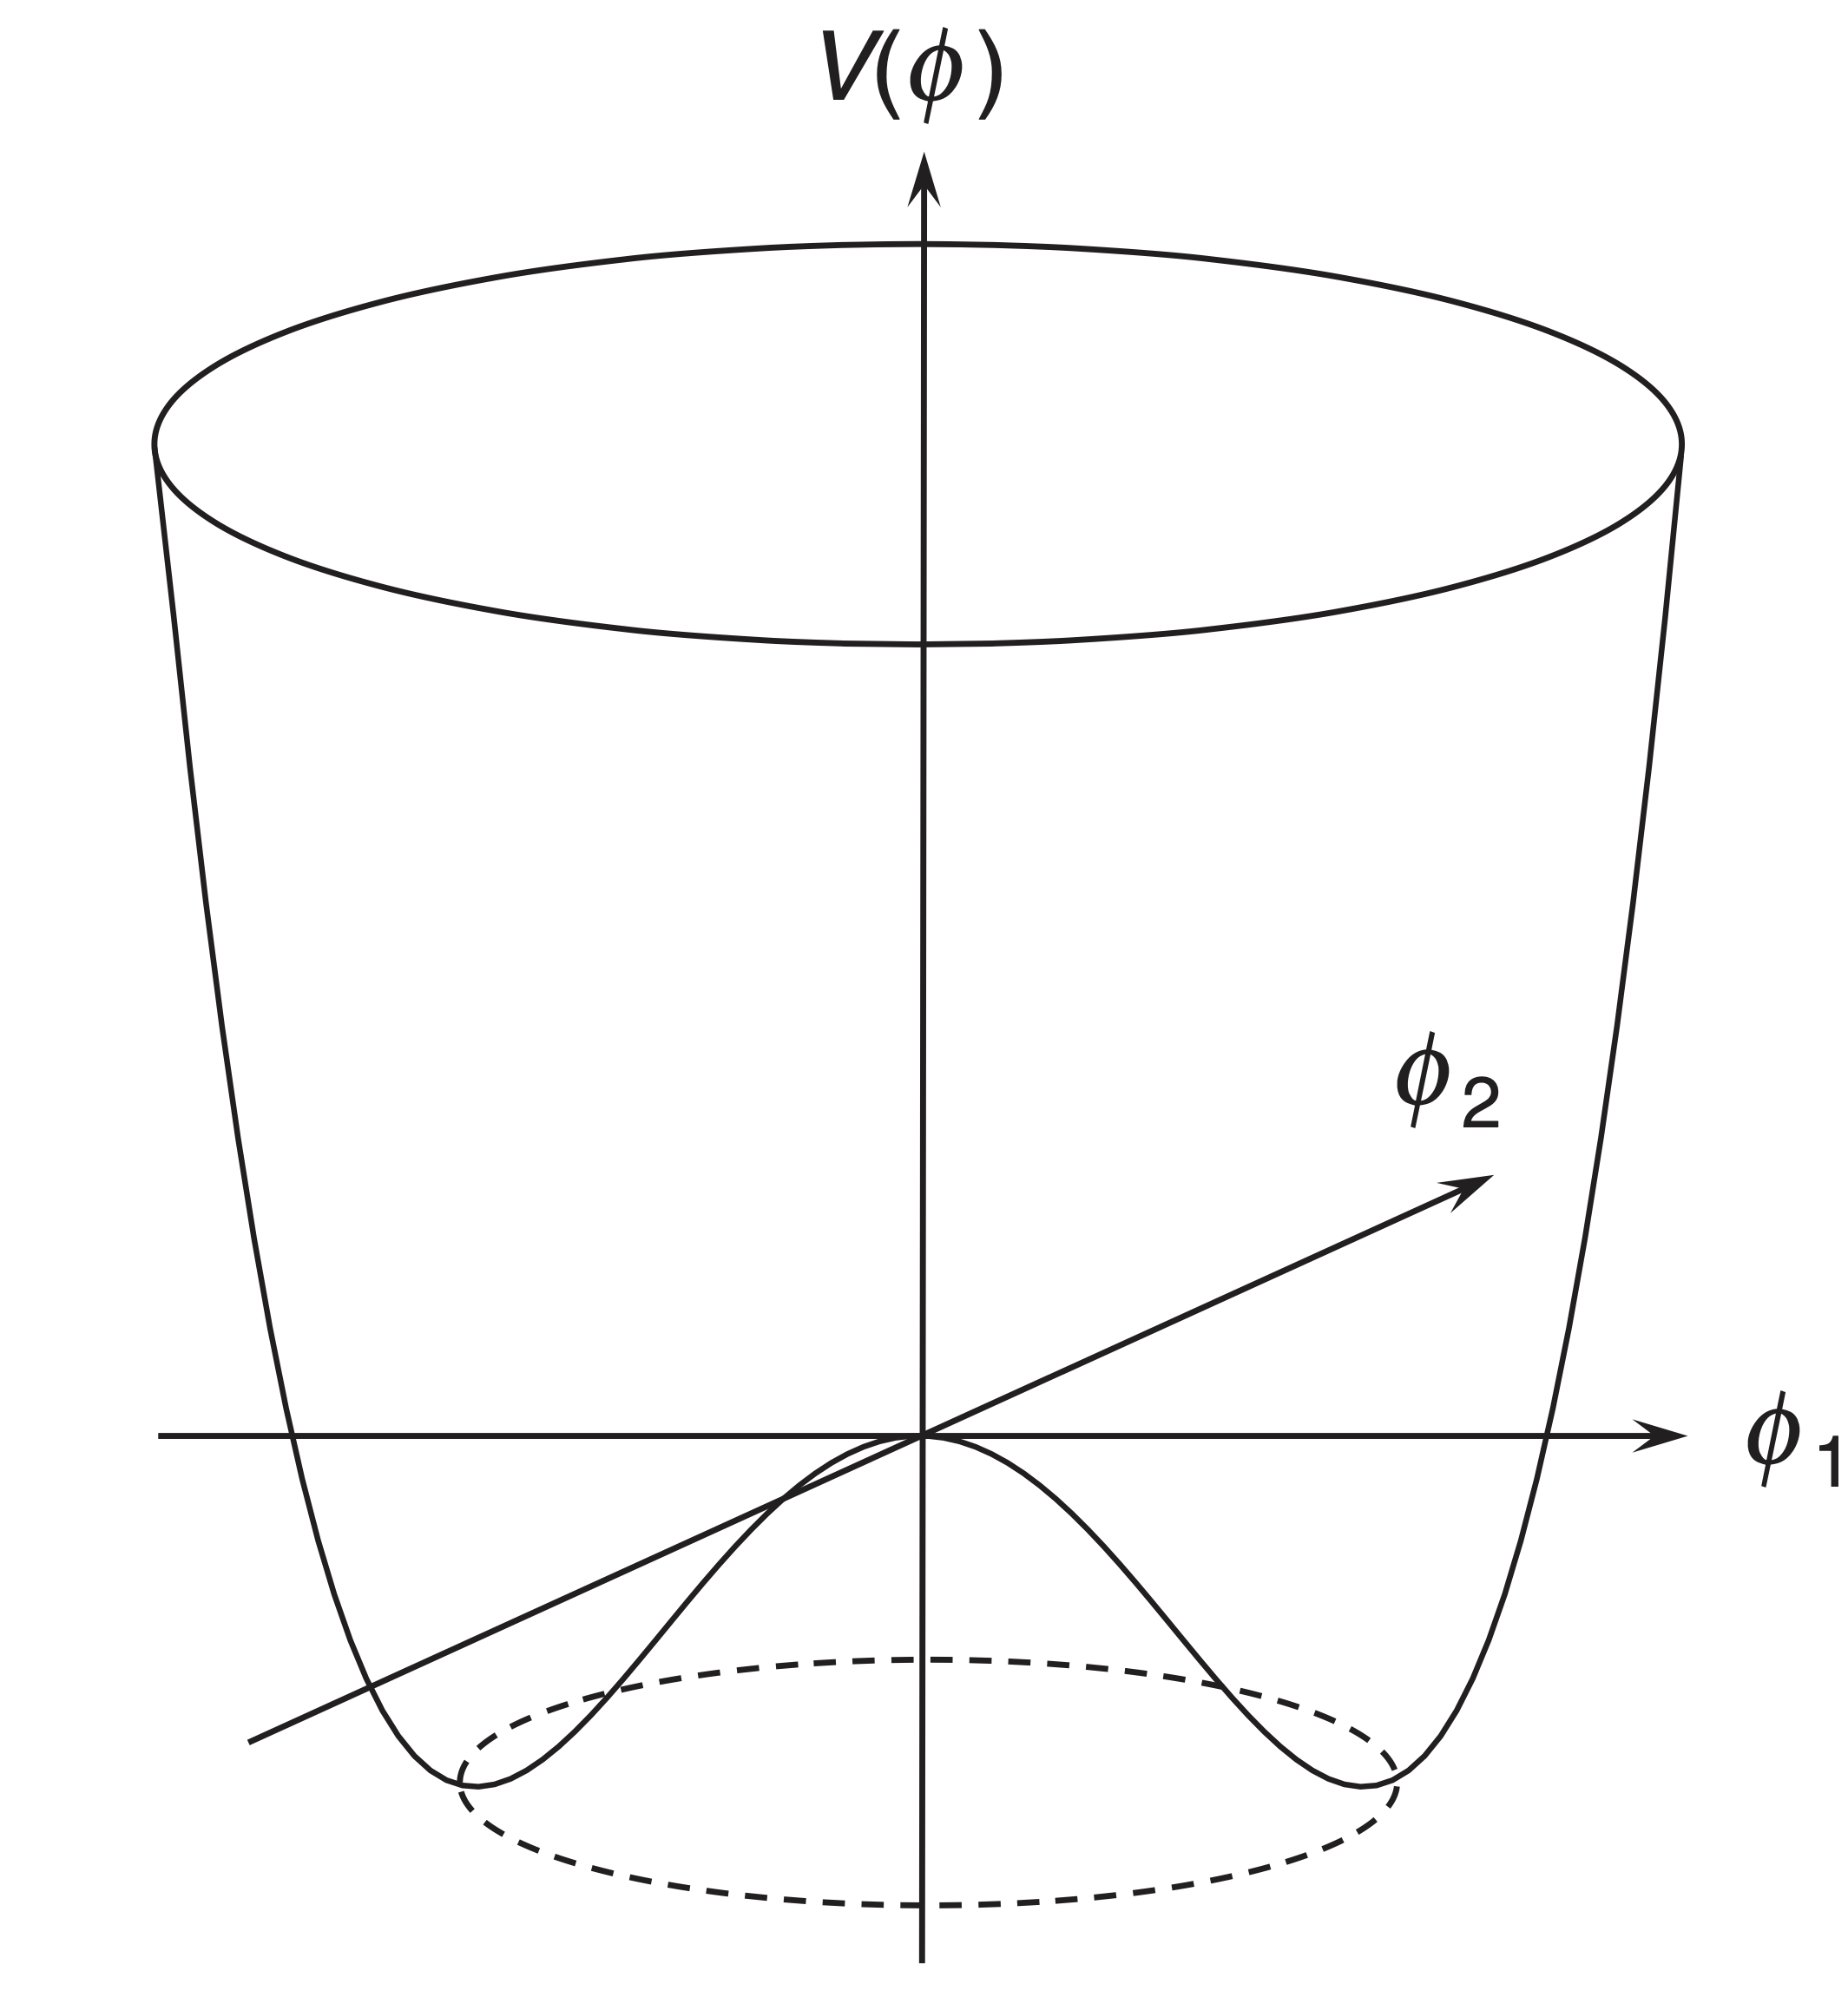
\includegraphics[width=.5\textwidth]{Images/HiggsPotential.png}
    \caption{A graph of the Higgs potential $V(\phi)$ as a function of the complex scalar Higgs field $\phi$ with real and imaginary components $\phi_1$ and $\phi_2$.}
    \label{fig:HiggsPotential}
\end{figure}
